\documentclass{article} % For LaTeX2e
\usepackage{nips12submit_e,times}
\usepackage{graphicx}
\usepackage{algorithmic}
\usepackage[ruled,vlined]{algorithm2e}
\usepackage{dsfont}
%\documentstyle[nips12submit_09,times,art10]{article} % For LaTeX 2.09
%\DeclareMathOperator{\argmax}{argmax}
%\DeclareMathOperator*{\argmin}{argmin}
%\DeclareMathOperator*{\Corr}{Corr}
\newcommand{\R}{\ensuremath{\mathds{R}}}
\usepackage{hyperref}
\title{Predicting political party affiliation\\ from parliament speeches}


\author{
Felix Bie\ss{}mann\thanks{} \\
\texttt{felix.biessmann@gmail.com} \\
\And
Daniel Kirsch\thanks{}\\
\texttt{mail@danielkirs.ch} \\
}
% The \author macro works with any number of authors. There are two commands
% used to separate the names and addresses of multiple authors: \And and \AND.
%
% Using \And between authors leaves it to \LaTeX{} to determine where to break
% the lines. Using \AND forces a linebreak at that point. So, if \LaTeX{}
% puts 3 of 4 authors names on the first line, and the last on the second
% line, try using \AND instead of \And before the third author name.

\newcommand{\fix}{\marginpar{FIX}}
\newcommand{\new}{\marginpar{NEW}}

\nipsfinalcopy % Uncomment for camera-ready version

\begin{document}


\maketitle

\begin{abstract}
Political parties are typically characterized by the opinions they represent. These political views are subject of the debates in political parliaments. We used the text of speeches and discussions in the German parliament to train a classifier that predicts the political party affiliation based on standard text features. We evaluate the classifier on parliament speeches and party manifestos. Results indicate that automatic classification of political affiliation is possible to some extent. We show how such a classifier can then be used to assess the political affiliation of authors of news articles or lobby groups. 
\end{abstract}

\section{Introduction}


\section{Methods}
We extracted the texts from the official webpage of the German parliament\footnote{\url{http://www.bundestag.de/plenarprotokolle}}. The texts were split using regular expressions and party labels were extracted from the texts. The number of speeches for each political party is listed in \autoref{tab:results}. Strings of teach speech are extracted using a 5-gram bag-of-word vectorizer with subsequent hashing to a vector $x\in\mathds{R}^d$, were $d$ is just about $10^6$, as implemented in scikit-learn \cite{scikit-learn}. 

\section{Results}

Wallclock time: 1319.548865 sec
Vocabulary size: 1048576
%
\begin{table}[t]
\begin{center}
\begin{tabular}{clrrrr}
&   \multicolumn{4}{c}{Predicted}\\
\multirow{ 2}{*}{True} & linke & 1422 & 371 &  43&  182\\
 & 144& 2188  & 44 & 198\\
 [  29   94 1663  413]
 [  60  131  101 2937]]
%
\end{tabular}
\end{center}
\caption{
\label{tab:results}
Some results.
}
\end{table}
\begin{table}[t]
\begin{center}
\begin{tabular}{lrrrr}
    &         precision    &recall &  f1-score  & N\\
\hline \hline
      linke     &  0.86    &  0.70  &    0.77   &   2018\\
     gruene   &    0.79    &  0.85   &   0.82 &     2574\\
        spd     &  0.90    &  0.76   &   0.82  &    2199\\
        cdu    &   0.79    &  0.91  &    0.84  &    3229\\
\hline
avg / total    &   0.83  &    0.82  &    0.82 &    10020\\
%
\end{tabular}
\end{center}
\caption{
\label{tab:results}
Some results.
}
\end{table}
%
%
\begin{figure}
\centering
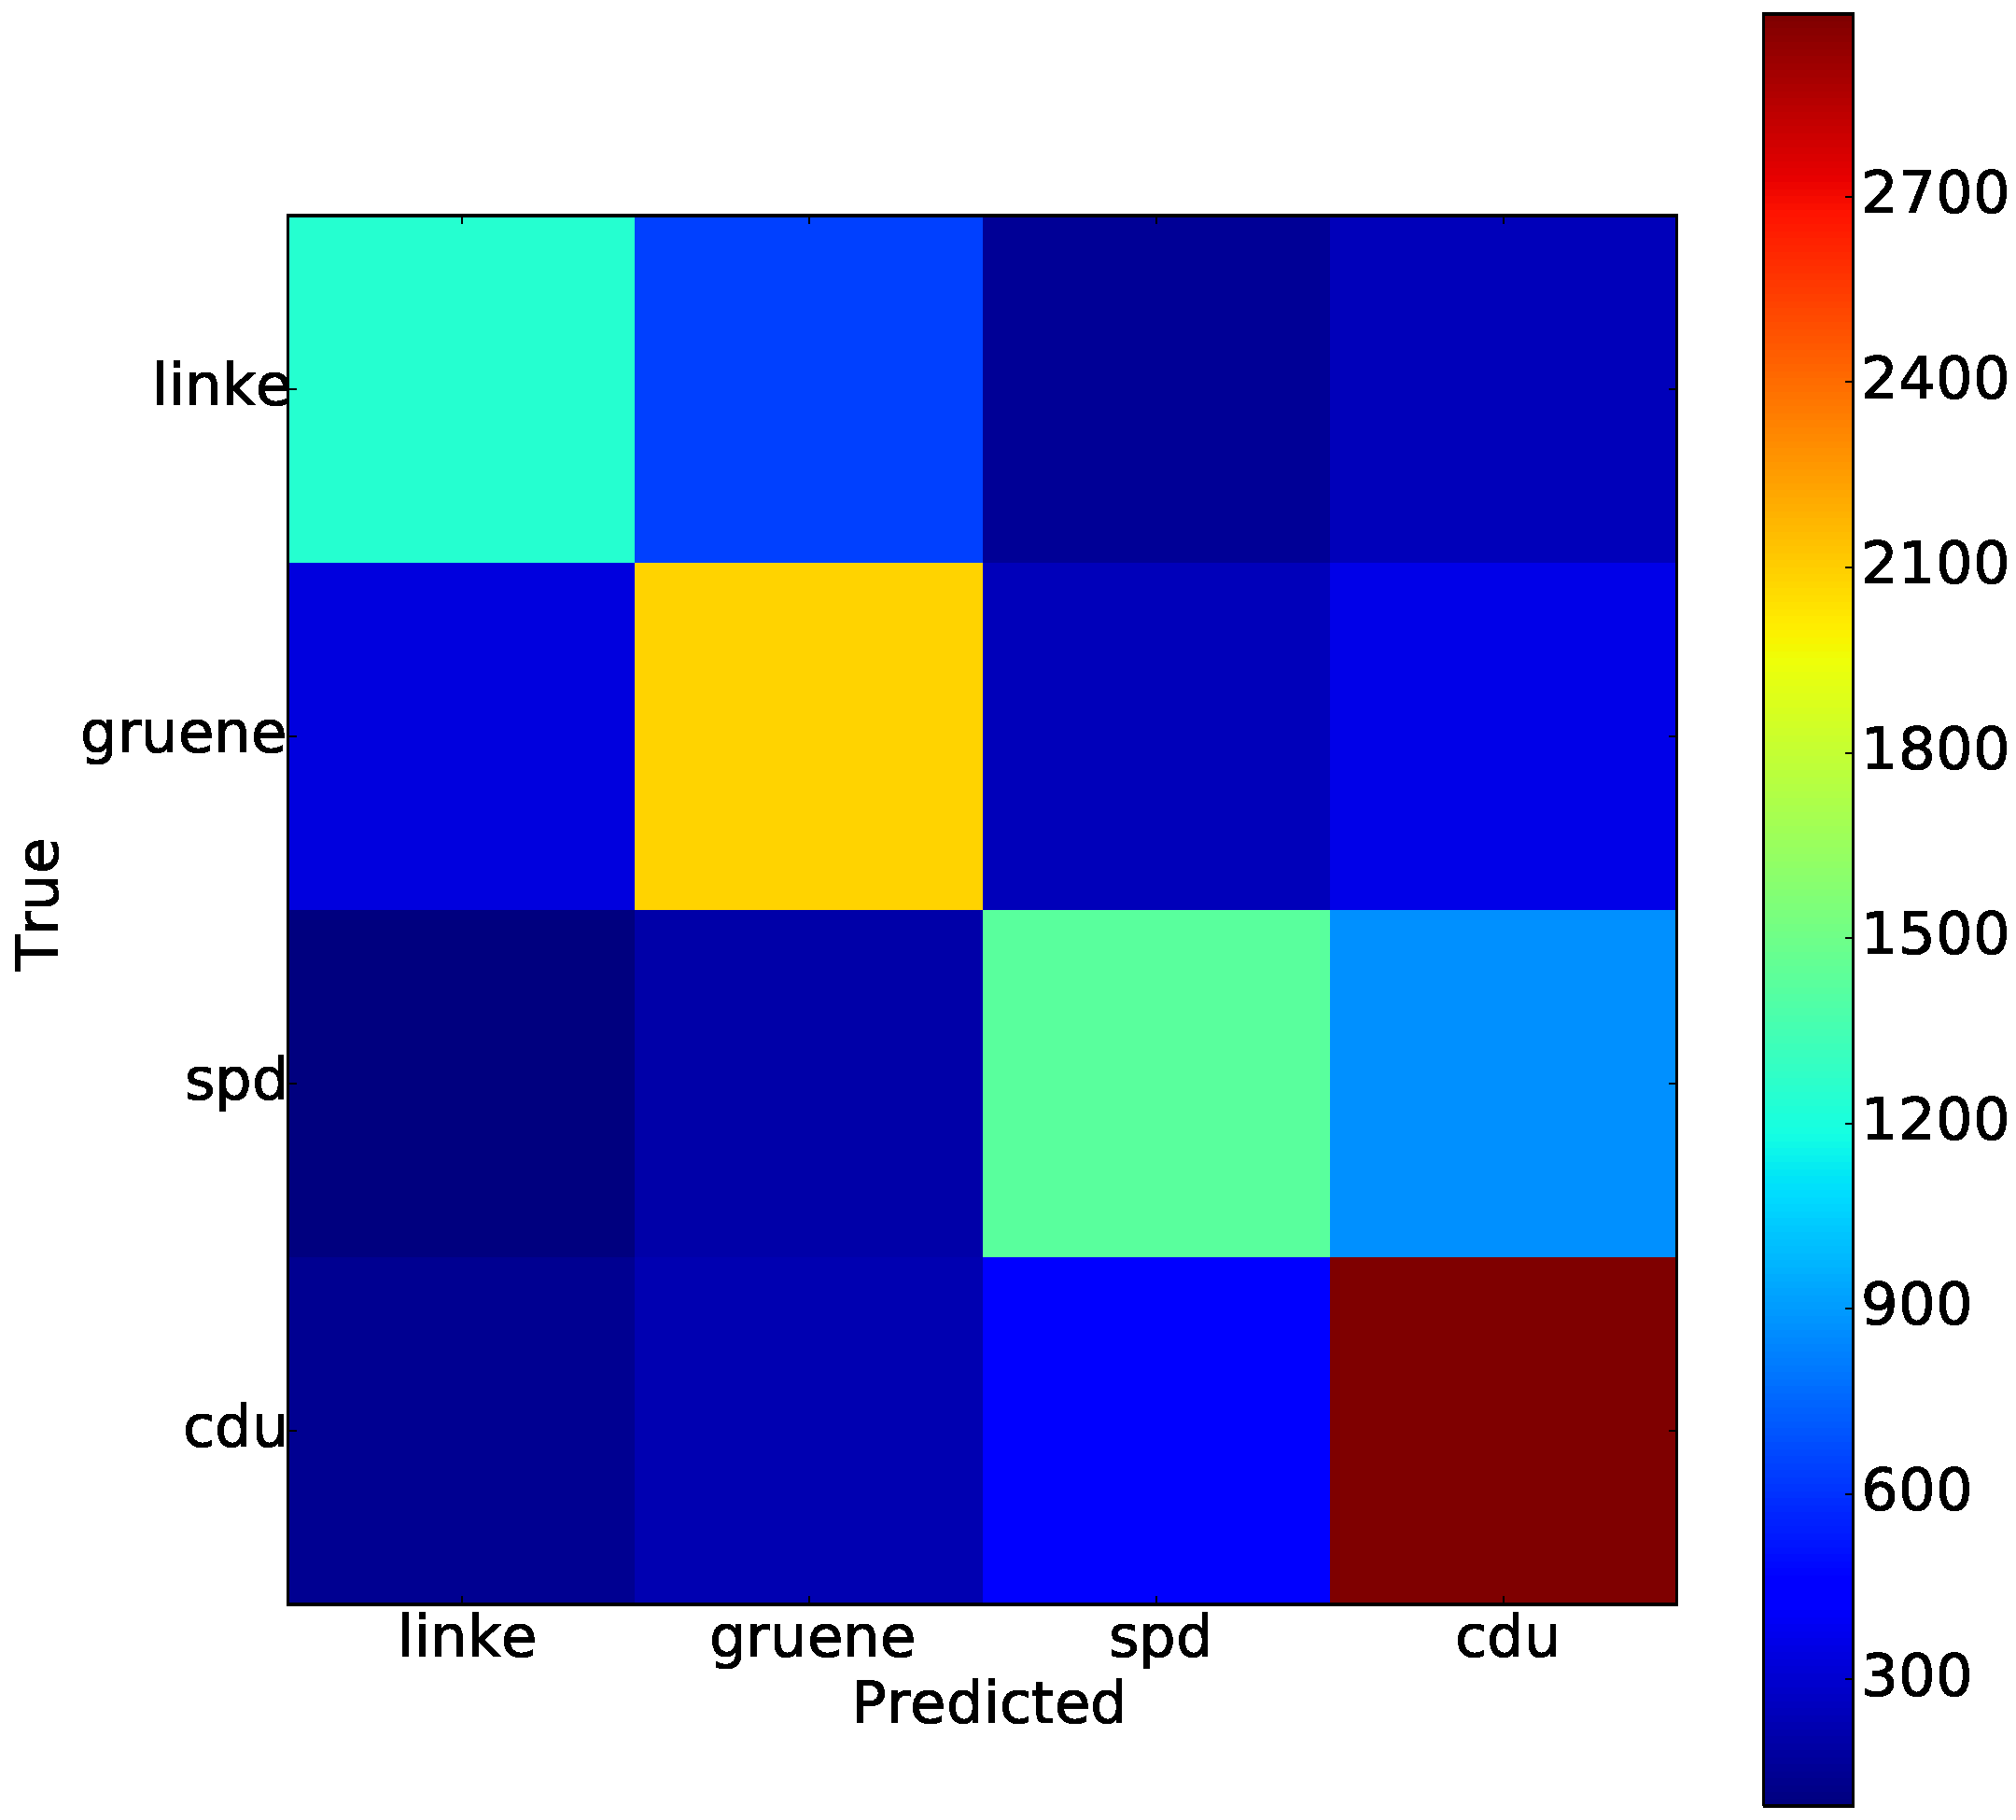
\includegraphics[width=.4\textwidth]{conf_mat}
\caption{\label{fig:confusion_matrix}
\small
}
\end{figure}
%

\paragraph{Word-Party Patterns}
11656 speeches, 74650 words (after stopword filtering)

\section{Conclusion}

\small{
\bibliographystyle{plain}
\bibliography{bibliography} 
}

\end{document}
